\pagebreak

\section{Views}
\subsection{Logical view}

\begin{figure}[H]
%\vspace{-30pt}
\begin{center}
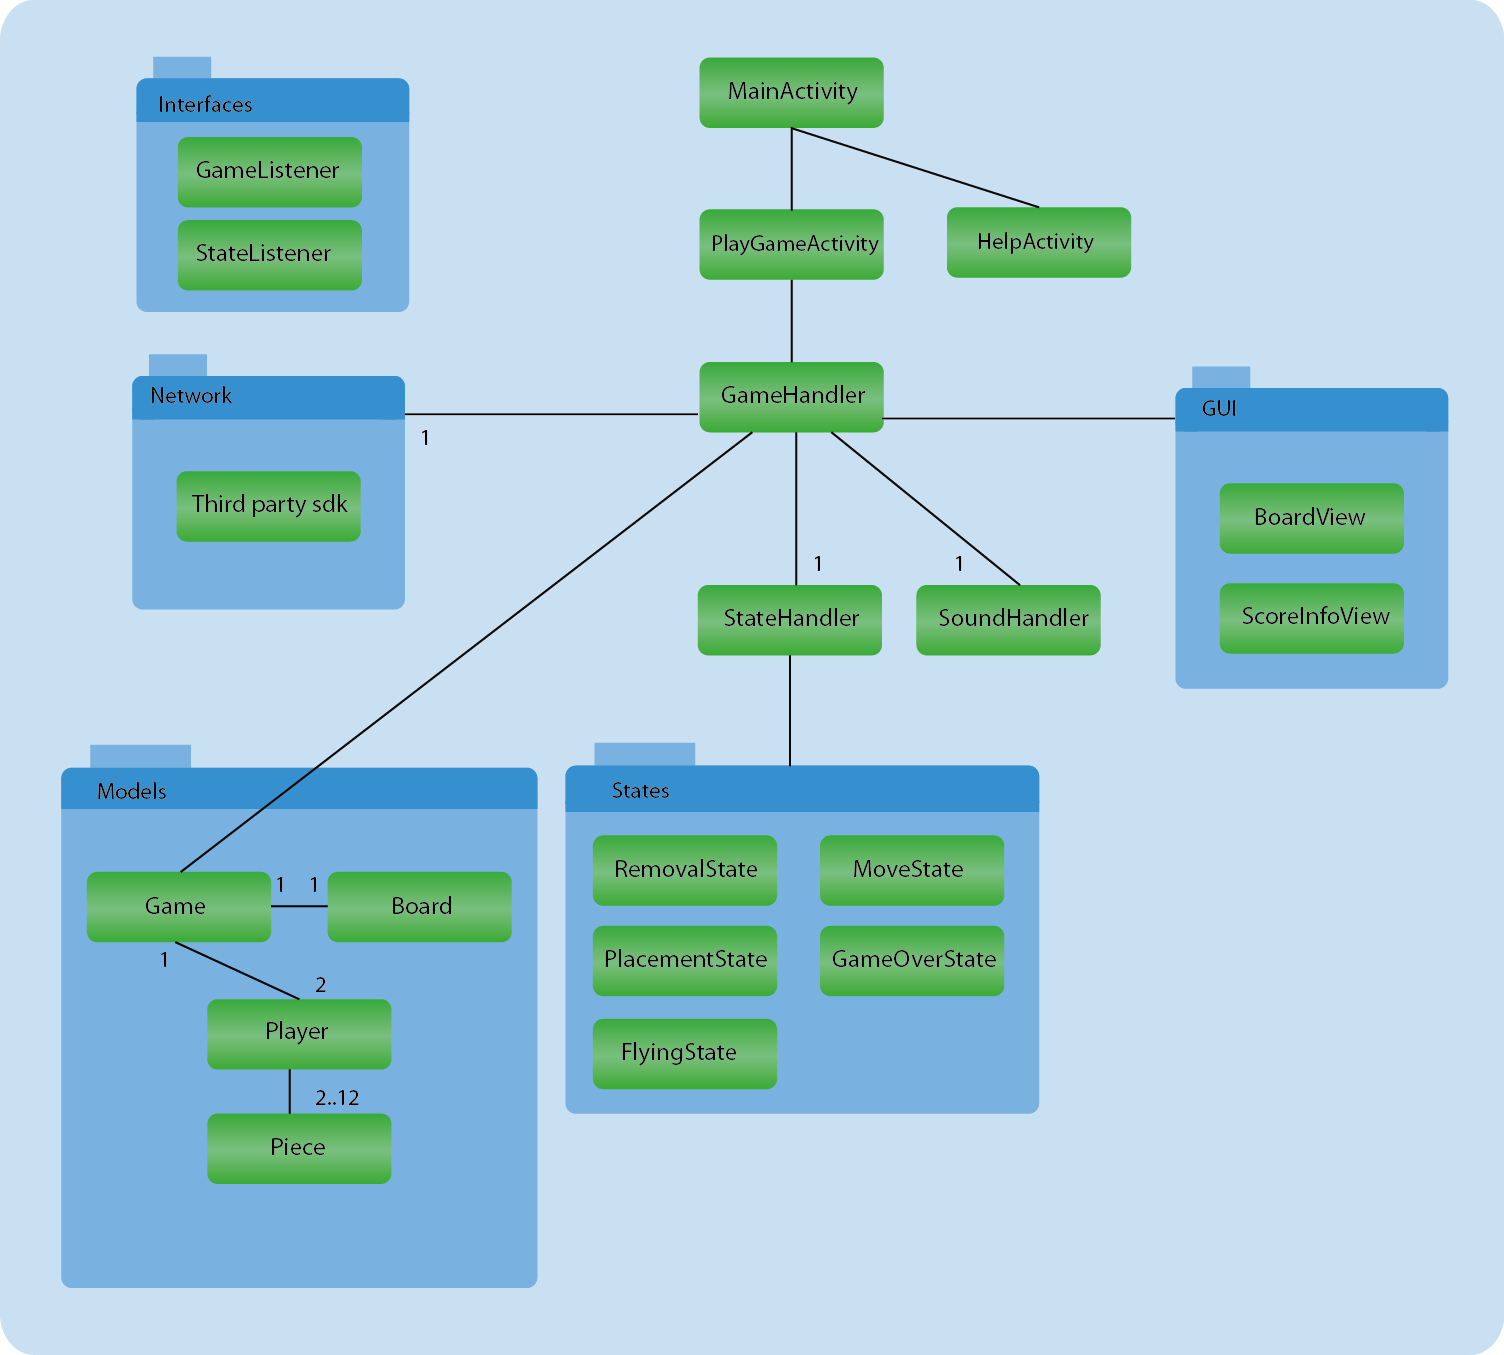
\includegraphics[width=\textwidth]{./Images/LogicalView.png}
\end{center}
\caption{Logical view}
\end{figure}

The diagram follows the 4+1 logic view notation suggested by the Kructhen article \cite{krutchen}. The class diagram shows the structure of a system by showing the system's classes  and the relationships among them. Aggregation and inheritance is also displayed.

\subsection{Development view}

\begin{figure}[H]
\begin{center}
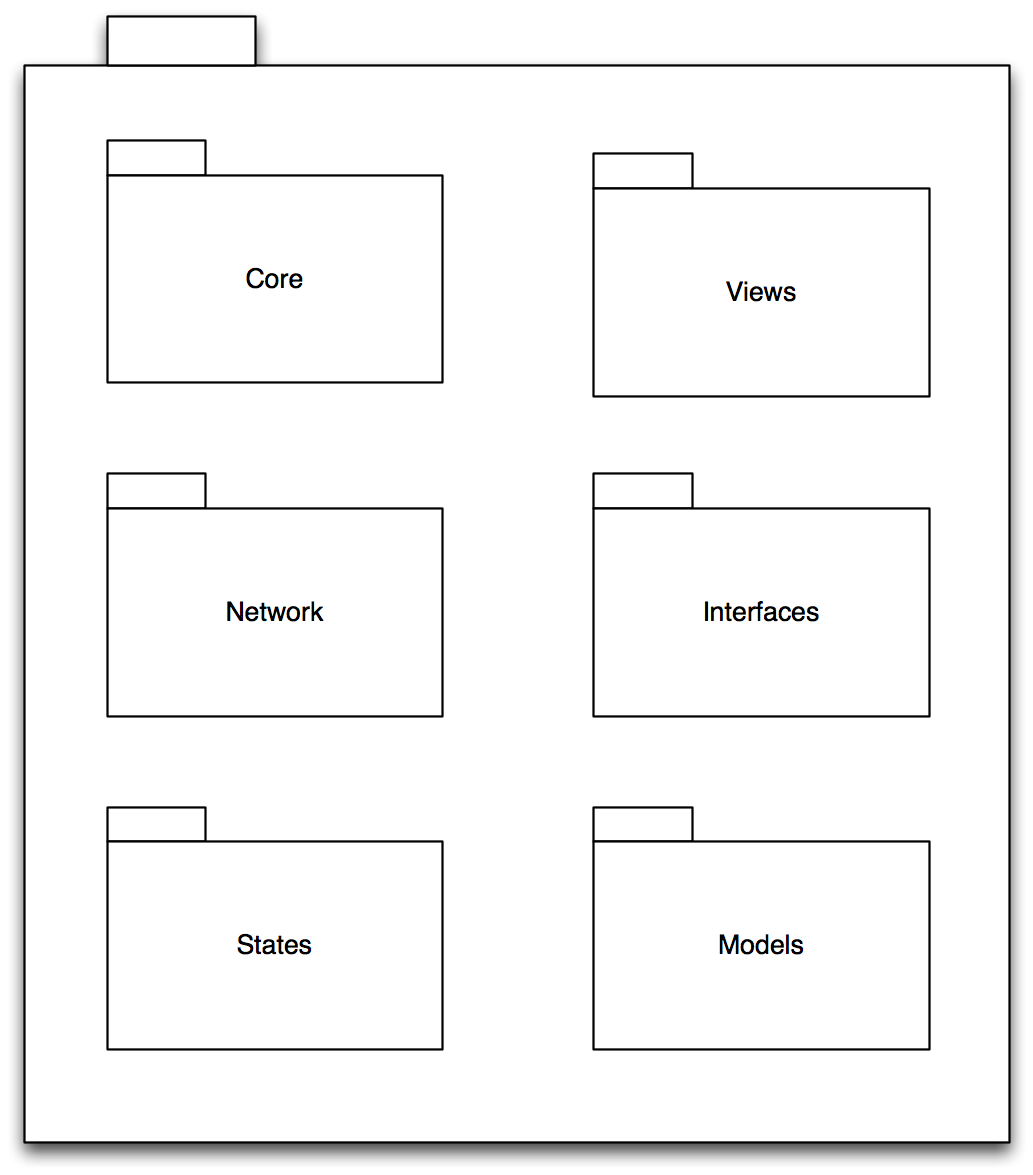
\includegraphics[width=220pt]{./Images/DevelopmentView.png}
\end{center}
\caption{Development view}
\end{figure}

The game is divided into several layers. The android framework, a 2D framework, the game logic, and graphics. The diagram show the different parts of the system.

\pagebreak

\subsection{Process view}

\begin{figure}[H]
%\vspace{-30pt}
\begin{center}
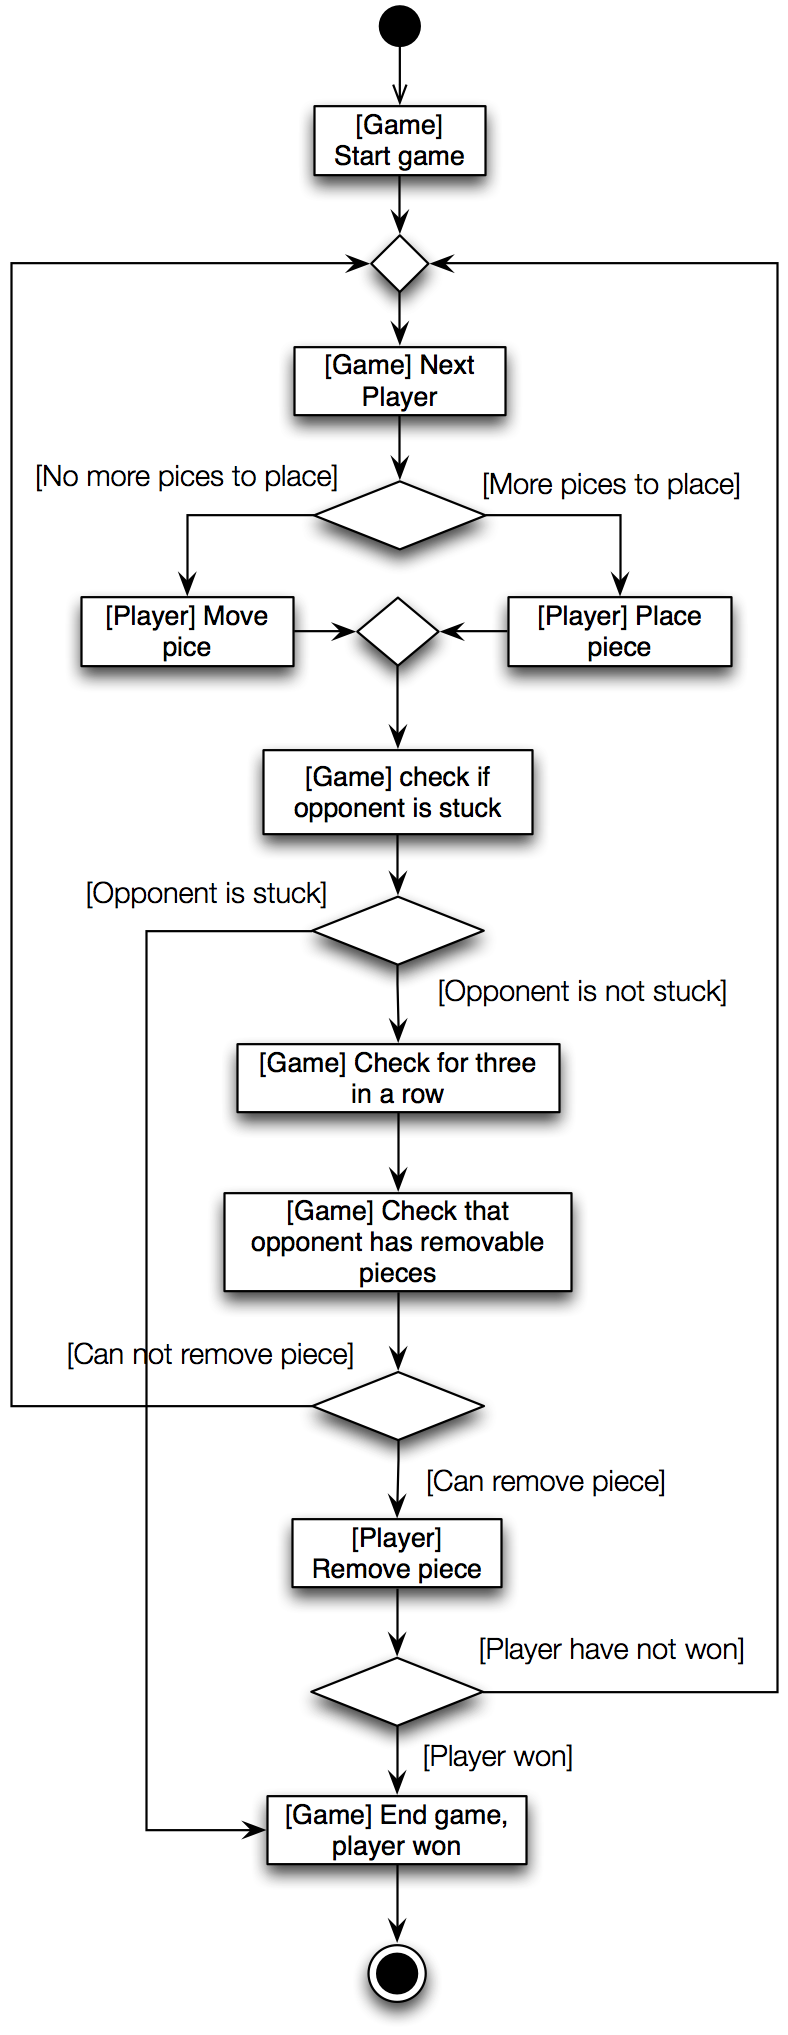
\includegraphics[width=200pt]{./Images/ProcessView}
\end{center}
\caption{Process view}
\end{figure}

The game is a turn based game with two players. In the activity diagram the progress of a game is described. When a game is started one of the players starts placing one of its pieces. The game checks if the player get three in a row. In that case the player can remove one of the opponents pieces. If the opponents have less then three pieces left, the other player have won. The diagram shows how a game round will pan out. 




